%------------------------------------------------
\section{Introduction on epidemiology}
%------------------------------------------------
\begin{frame}[t]
	\frametitle{Research displinces in epidemiology}
	\tikzstyle{background grid}=[draw, black!50,step=.5cm]
	%
	Forecasting novel epidemics is a multidisciplinary field involving multiple \emph{targets} \ifshowcitations\footpartcite{Wu2021}\fi\\
	~\\
	\begin{columns}
		\begin{column}{0.5\textwidth}
			In the early stages of epidemics, we have access to:\\
			%
			\begin{itemize}
				\item<2-> \only<2>{\emphasis}{Social behaviour and demographics}
				\item<3-> \only<3>{\emphasis}{Incidence rate data}
			\end{itemize}
			%
			Simulation models can be developed based on this information and used in \only<4>{\emphasis}{public health and social measures (PHSMs)} policy-making.
		\end{column}
		\begin{column}{0.5\textwidth}
			\begin{tikzpicture}[remember picture, overlay] %show background grid, 
				% Put the graphic inside a node. This makes it easy to place the
				% graphic and to draw on top of it. 
				% The above right option is used to place the lower left corner
				% of the image at the (0,0) coordinate. 
				\node [inner sep=0pt,above left, opacity=1.0]  at (0.99\textwidth,-0.5\textheight) (targets) 
					{
						\only<1>{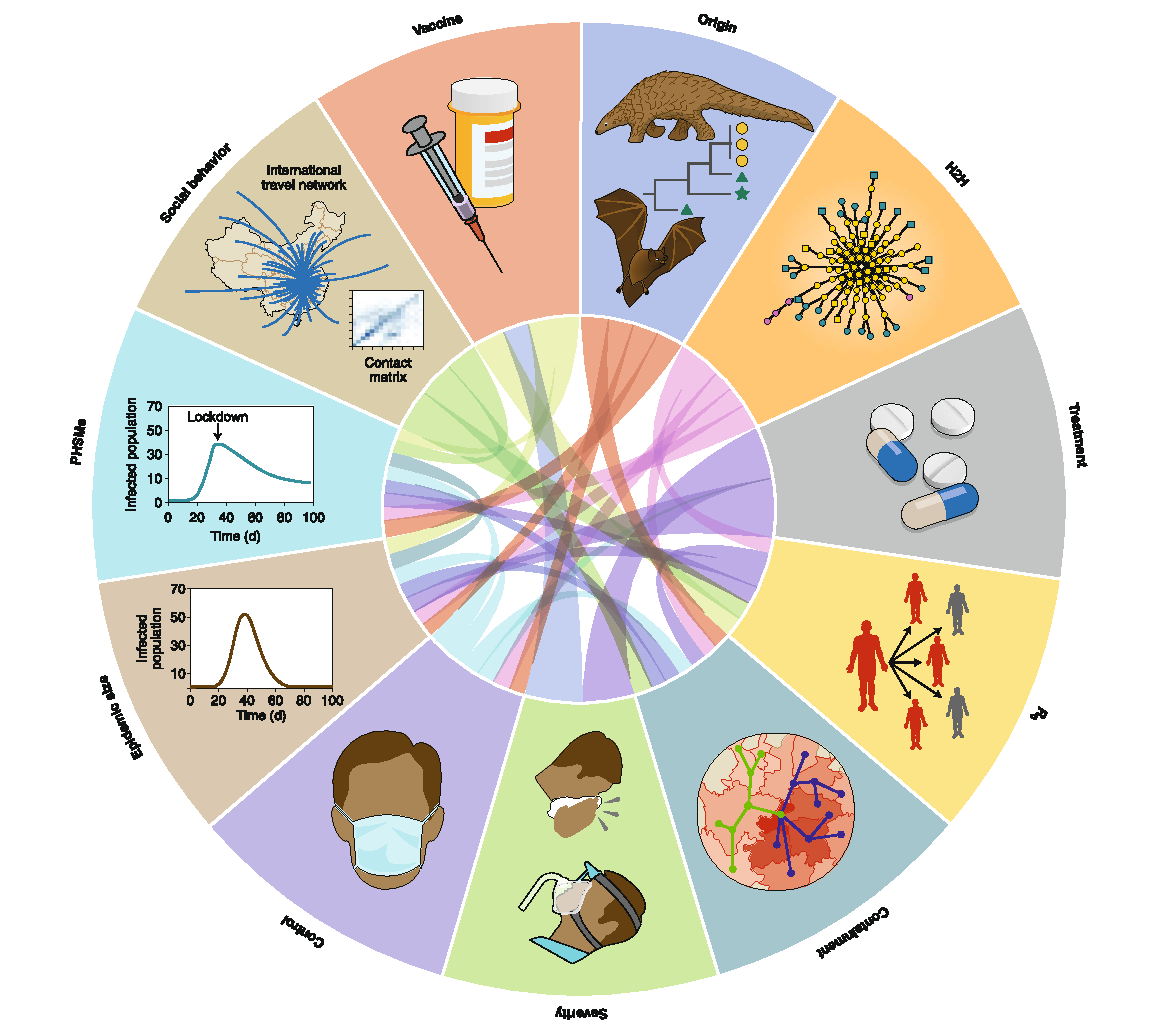
\includegraphics[width=0.9\textwidth]{targets/nowcasting_targets_1.pdf}}%
						\only<2>{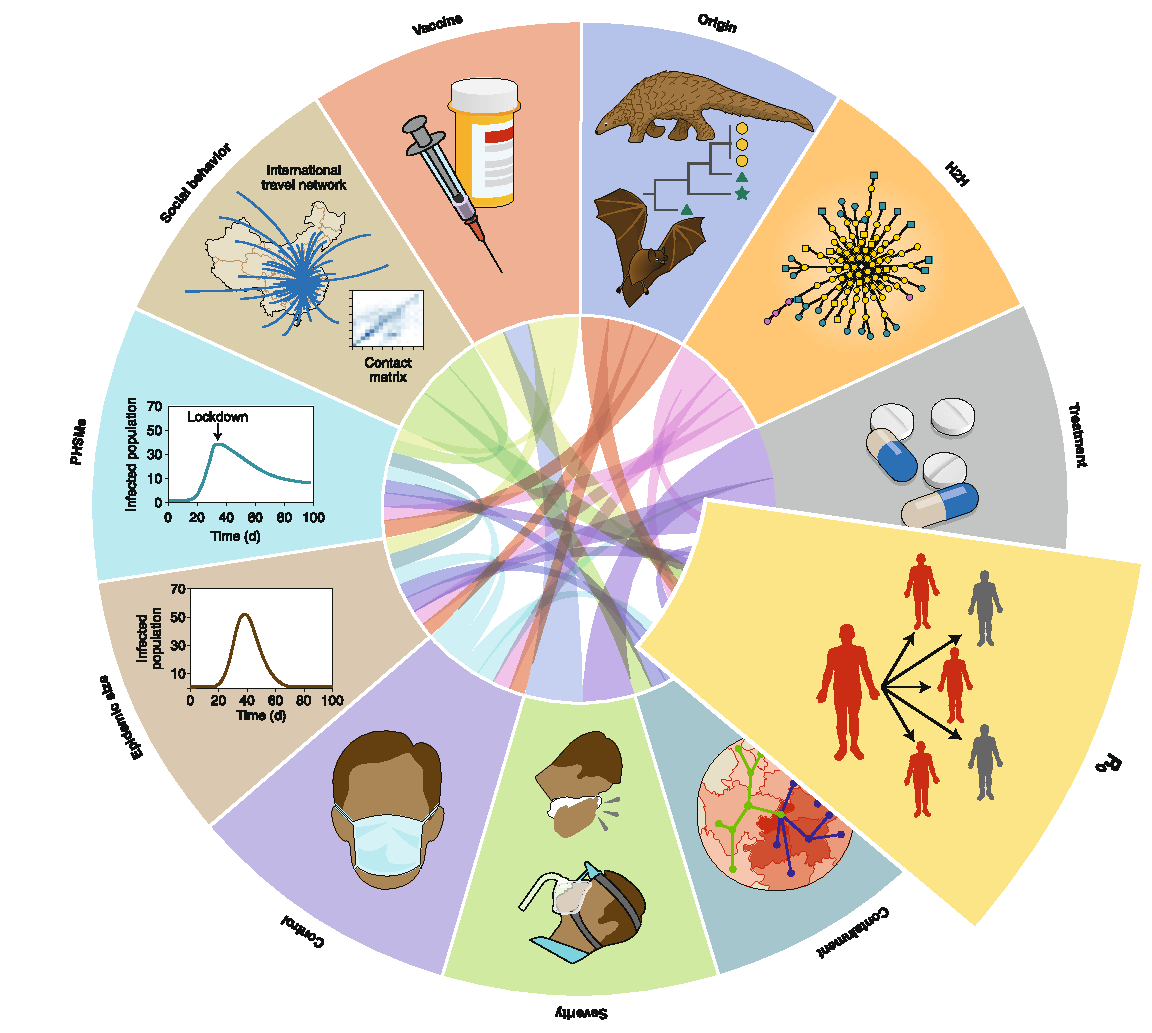
\includegraphics[width=0.9\textwidth]{targets/nowcasting_targets_2.pdf}}%
						\only<3>{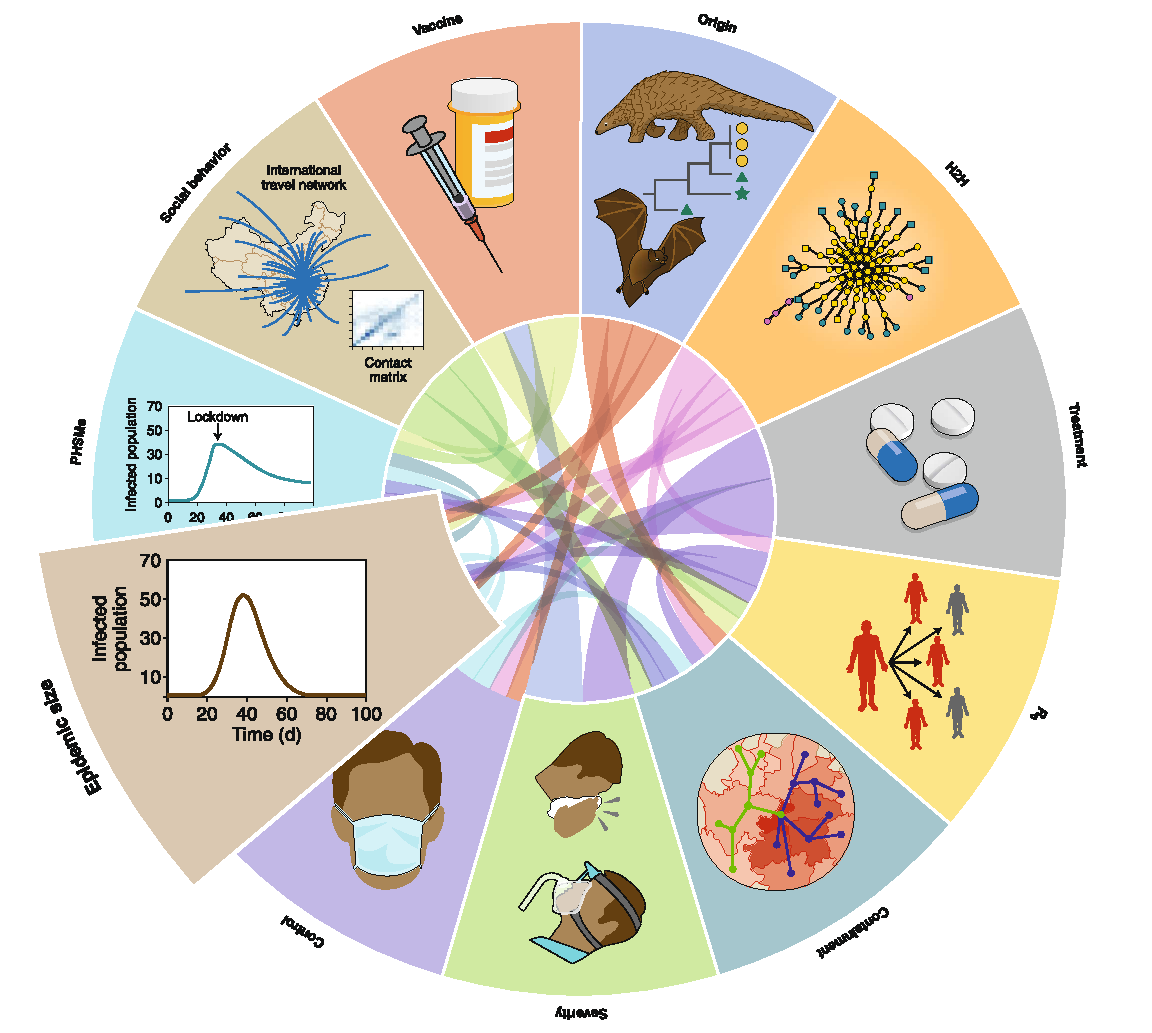
\includegraphics[width=0.9\textwidth]{targets/nowcasting_targets_3.pdf}}%
						\only<4->{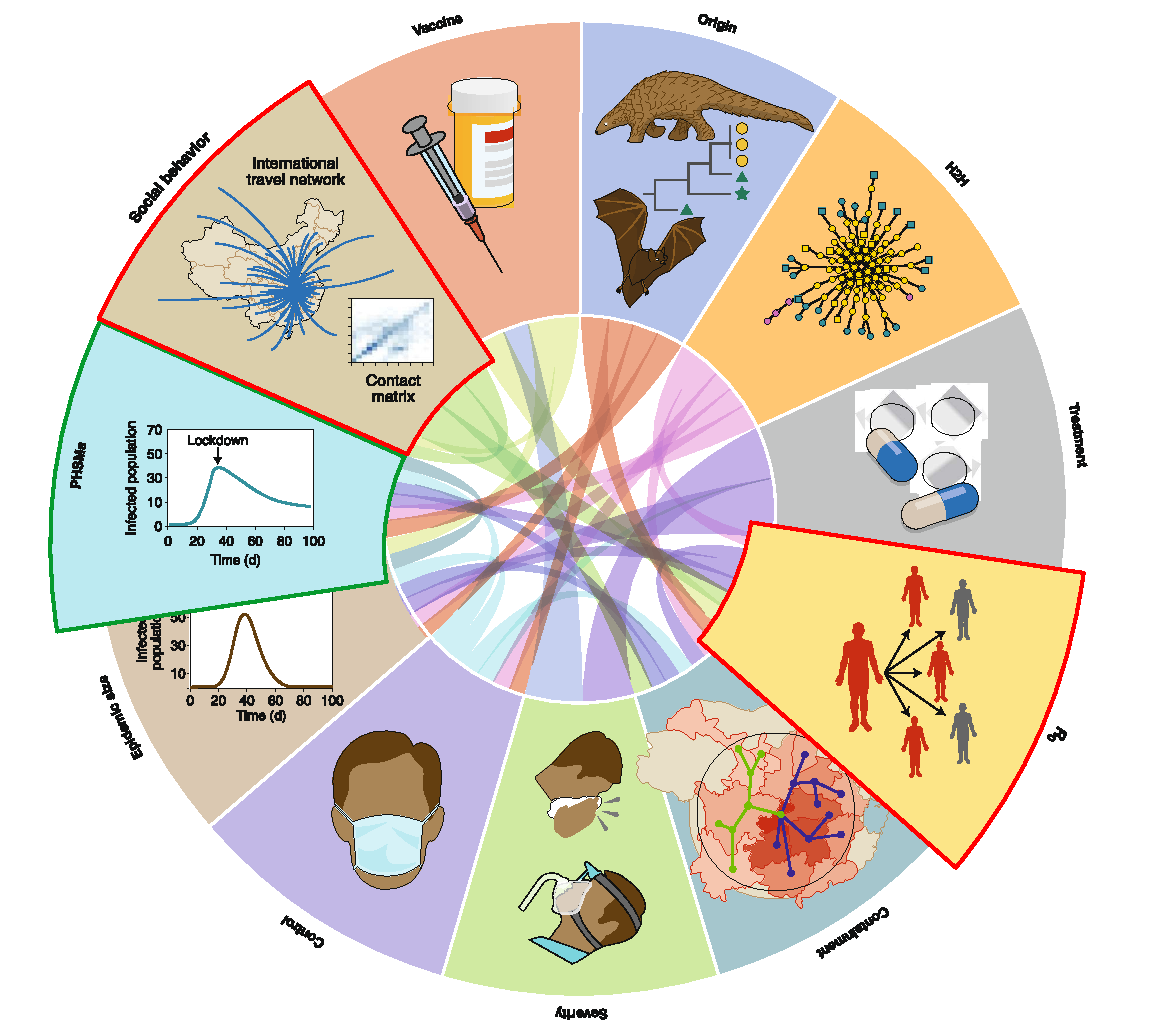
\includegraphics[width=0.9\textwidth]{targets/nowcasting_targets_4.pdf}}%
					};
				% show origin
				% \fill (0,0) circle (2pt);
			\end{tikzpicture}%
		\end{column}
	\end{columns}
	%
	\vspace{-3em}
\end{frame}
\addtocounter{footnote}{-1}
%------------------------------------------------
\begin{frame}[c,noframenumbering]
	\centering
	% \setlength\fboxsep{0pt}
	\begin{titleblock}{}
		\centering 
		~\\%
		{\centering\LARGE Simulation and modeling of pandemics in early stages\ifshowcitations\footnotemark[1]\fi\\}%
		~\\%
		{\textit{Joint work with: Prof. Michael Kokkolaras}}
	\end{titleblock}
	{\color{white}\ifshowcitations\footpartcite{Alhandawi2021b}[1]\fi}
\end{frame}
\addtocounter{footnote}{-1}
%------------------------------------------------